\documentclass{article}
\usepackage{graphicx}
\usepackage{fancyhdr}
\usepackage{listings}

\let\<\textless
\let\>\textgreater

\graphicspath{ {images/} }
\pagestyle{fancy}
\fancyhf{}
\rhead{Bases de datos geoespaciales}
\rfoot{P\'agina \thepage}

\begin{document}
\begin{titlepage}
  \centering
  {\scshape\LARGE Instituto Tecnol\'ogico de Costa Rica \par}
  \vspace{1cm}
  {\scshape\Large Bases de datos geoespaciales\par}
  \vspace{1.5cm}
  {\Large\itshape Alejandro Rojas\par}
  {\Large\itshape Sa\'ul Zamora\par}
  \vfill
  profesor\par
  Kevin Moraga \textsc{}

  \vfill

% Bottom of the page
\end{titlepage}

\section{Bases de datos espaciales}
Las bases de datos espaciales son bases de datos optimizadas para almacenar datos que representan objetos definidos sobre un espacio geom\'etrico y realizar consultas sobre dichos datos. La mayor\'ia de las bases de datos espaciales permiten representar objetos geom\'etricos simples como puntos, lineas y pol\'igonos. Algunas permitan el manejo de estructuras m\'as complejas como objetos 3D, coberturas topol\'ogicas, redes lineares y redes irregulares trianguladas.
Mientras que las bases de datos tradicionales han sido desarrolladas para manejar m\'ultiples tipos de datos num\'ericos y de caract\'eres, dichas bases de datos requieren funcionalidad adicional para procesar datos espaciales eficientemente y generalmente se agregan tipos de datos como \emph{geometry} o \emph{feature} para manejar datos espaciales.

\section{Consultas espaciales}
Consultas espaciales son el tipo de consulta manejada por los sistemas de bases de datos espaciales. Dichas consultas difieren de las no-espaciales en dos aspectos importantes:
\begin{itemize}
  \item Las consultas espaciales usan datos geom\'etricos como puntos, l\'ineas y pol\'igonos.
  \item Estas consultas consideran la relaci\'on espacial entre las geometr\'ias mencionadas.
\end{itemize}

\section{Tipos de consultas espaciales}
Los nombres de funciones para consultas difieren de un sistema a otro. La siguiente lista contiene funciones com\'unmente a\~nadidas a \emph{PostGIS}, el cual es una extensi\'on de PostgreSQL para el manejo de datos espaciales (el t\'ermino \emph{geometry} se refiere a un punto, l\'inea, caja u otra figura de 2 o 3 dimensiones):

\begin{itemize}
  \item Distance(geometry, geometry) : number
  \item Equals(geometry, geometry) : boolean
  \item Disjoint(geometry, geometry) : boolean
  \item Intersects(geometry, geometry) : boolean
  \item Touches(geometry, geometry) : boolean
  \item Crosses(geometry, geometry) : boolean
  \item Overlaps(geometry, geometry) : boolean
  \item Contains(geometry, geometry) : boolean
  \item Length(geometry) : number
  \item Area(geometry) : number
  \item Centroid(geometry) : geometry
\end{itemize}

\section{Bases de datos geoespaciales}
Una base de datos geoespacial es una base de datos que almacena datos geogr\'aficos, tales como pa\'ises, divisiones administrativas, ciudades e informaci\'on relacionada. Dichas bases de datos pueden ser \'utiles para sitios web que deseen identificar la ubicaci\'on de sus visitantes con el fin de personalizar m\'as la visita.

\section{Caracter\'isticas de las bases de datos espaciales}
Los sistemas de bases de datos usan \'indices para buscar r\'apidamente valores y la forma en la que la mayor\'ia de sistemas indexan la informaci\'on no es \'optima para consultas espaciales. En lugar de eso, las bases de datos espaciales utilizan \'indices espaciales para acelerar las operaciones de base de datos.

Adicionalmente a las consultas t\'ipicas de SQL como \emph{SELECT}, las bases de datos espaciales pueden realizar una amplia variedad de operaciones espaciales:

\begin{itemize}
  \item Medidas espaciales: procesa largo de l\'ineas, \'areas poligonales, distancias entre geometr\'ias, etc.
  \item Funciones espaciales: modificar las caracter\'isticas existentes de un objeto para crear nuevas, por ejemplo, agregando un buffer alrededor de un objeto, etc.
  \item Predicados espaciales: permite consultas de falso\/verdadero sobre relaciones entre objetos, como la superposici\'on de un objeto sobre otro, la ubicaci\'on de un punto dentro de un \'area.
  \item Constructores geom\'etricos: creaci\'on de nuevas geometr\'ias, usualmente mediante la especificaci\'on de los v\'ertices que definen la figura.
  \item Funciones de observaci\'on: consultas que retornan informaci\'on espec\'ifica sobre una figura, como la ubicaci\'on del centro de un c\'irculo.
\end{itemize}

Algunas bases de datos soportan solo versiones simplificadas o modificadas de estas operaciones, especialmente en casos como los de sistemas NoSQL como MongoDB y CouchDB.

\section{\'Indices espaciales}
Los \'indices espaciales son los utilizados por las bases de datos espaciales para optimizar las consultas. Los \'indices convencionales no manejan las consultas espaciales de forma eficiente, tales como que tan lejos est\'a un punto de otro o si todos los puntos caen dentro de un \'area determinada. Los m\'etodos de indexaci\'on espacial m\'as com\'unes incluyen:

\begin{itemize}
  \item R-tree: m\'etodo preferido para la indexaci\'on de datos espaciales. Los objetos (formas, l\'ineas y puntos) son agrupados usando un \emph{rect\'angulo de enlace m\'inimo} o MBR por sus siglas en ingl\'es (\emph{Minimum Bounding Rectangle}). Los objetos se agregan al MBR dentro del \'indice, lo que lleva a que su tama\~no aumente de forma m\'inima.
  \item HHCode
  \item Grid
  \item Z-order
  \item Quadtree
  \item Octree
  \item UB-tree
  \item R+ tree
  \item R* tree
  \item Hilbert R-tree
  \item X-tree
  \item kd-tree
  \item m-tree
  \item M\'etodo de punto de acceso (\emph{Point access method})
  \item Particionamiento espacial binario o BSP-tree por sus siglas en ingl\'es \emph{Binary space partitioning}: subdividir el espacio en hiperplanos.
\end{itemize}

\begin{figure}[!ht]
  \caption{Ejemplo de R-tree para rect\'angulos bidimensionales}
  \centering
    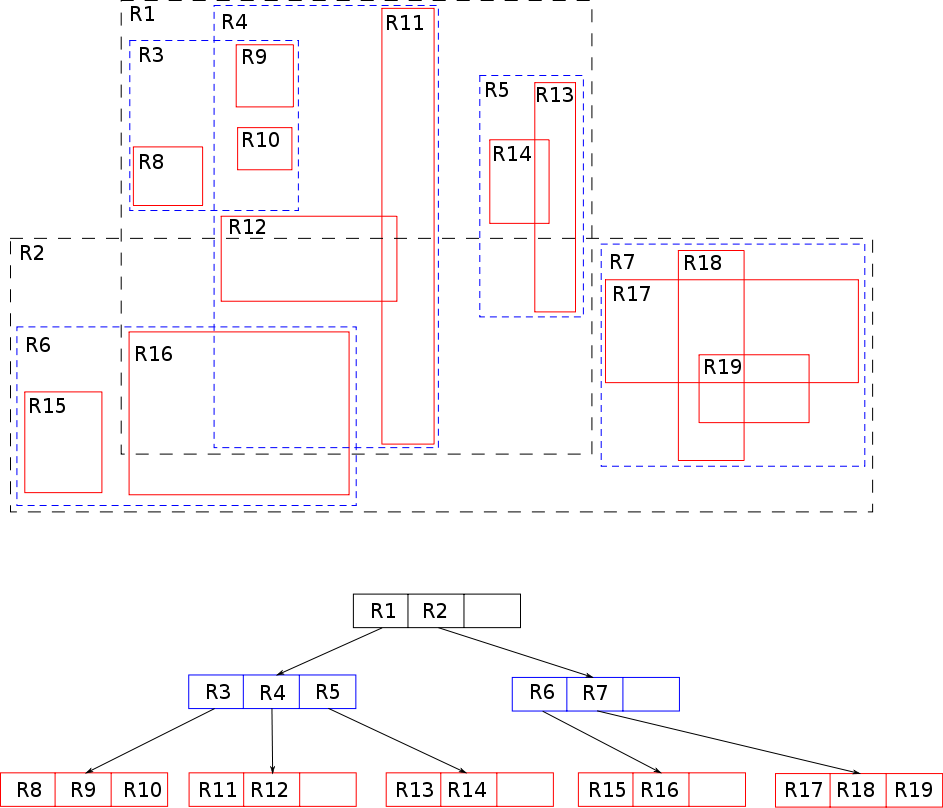
\includegraphics[width=0.4\textwidth]{r-tree.png}
\end{figure}

\begin{figure}[!ht]
  \caption{Visualizaci\'on de un R*-tree para puntos 3D}
  \centering
    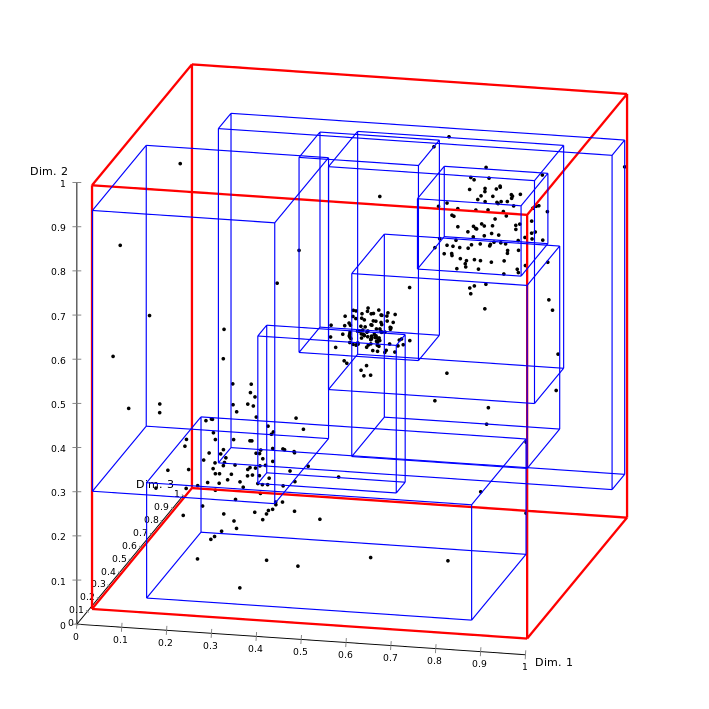
\includegraphics[width=0.4\textwidth]{3d-r-tree.png}
\end{figure}

\section{Usos de las bases de datos espaciales}
Uno de los usos m\'as populares para las bases de datos espaciales son los sistemas de informaci\'on geogr\'afica o GIS (por sus siglas en ingl\'es \emph{Geographic Information Systems}) son sistemas dise\~nados para capturar, almacenar, manupular, analizar, manejar y presentar datos espaciales o geogr\'aficos.

Estas aplicaciones permiten a los usuarios crear consultas interacticas, analizar informaci\'on espacial, editar datos en mapas y presentar los resultados de todas estas operaciones.

En los \'ultimos a\~nos han proliferado sistemas de libre uso con f\'acil acceso a software de mapeo, tales como Google Maps y OpenStreetMap. Dichos servicios dan al p\'ublico acceso a enormes cantidades de datos geogr\'aficos. Algunos de estos sistemas, como Google Maps, ofrecen al usuario APIs para crear aplicaciones m\'as personalizadas.

\begin{thebibliography}{99}
\bibitem{spatialdb}  En.wikipedia.org. (2017). Spatial database. [online] Available at: \texttt{https://en.wikipedia.org/wiki/Spatial\_database}

\bibitem{rtree} En.wikipedia.org. (2017). R-tree. [online] Available at: \texttt{https://en.wikipedia.org/wiki/R-tree}

\bibitem{gis} En.wikipedia.org. (2017). Geographic information system. [online] Available at: \texttt{https://en.wikipedia.org/wiki/Geographic\_information\_system}

\end{thebibliography}

\end{document}